
\textbf{Приклад 3.} Для графа $C_4$, зображеного на рисунку \ref{ex3:image}, порахуємо його спектр.\\
\begin{figure}[H]
    \centering
    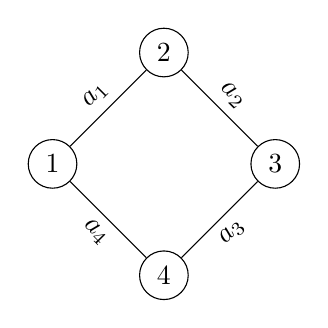
\begin{tikzpicture}[node distance={20mm}, main/.style = {draw, circle}]
    \node[main] (1) {$1$}; 
    \node[main] (2)[above right of=1] {$2$};
    \node[main] (3)[below right of=2] {$3$};
    \node[main] (4)[below left of=3] {$4$};
    \draw (1) -- node [midway, above, sloped] {$a_1$}(2);
    \draw (2) -- node [ above, midway, sloped] {$a_2$}(3);
    \draw (3) -- node [ below, midway, sloped] {$a_3$}(4);
    \draw (4) -- node [ below, midway, sloped] {$a_4$}(1);
    \end{tikzpicture}\\
    \caption{$C_4$}
    \label{ex3:image}
\end{figure}

Побудуємо матрицю суміжності $A$ для графа $C_4$ (рисунок \ref{ex3:image})

\begin{equation*}
A(G) =
\begin{pmatrix}
0 & a_1 & 0 & a_4\\
a_1 & 0 & a_2 & 0\\
0 & a_2 & 0 & a_3\\
a_4 & 0 & a_3 & 0
\end{pmatrix}
\end{equation*}

Знайдемо характеристичний многочлен за формулою (\ref{eq1})

\begin{multline*}
    P({\bf G})= 
\begin{vmatrix}
    \lambda & -a_1 & 0 & -a_4\\
    -a_1 & \lambda & -a_2 & 0\\
    0 & -a_2 & \lambda & -a_3\\
    -a_4 & 0 & -a_3 & \lambda
\end{vmatrix}
= \\
=\lambda
\begin{vmatrix}
    \lambda & -a_2 & 0\\
    -a_2 & \lambda & -a_3\\
    0 & -a_3 & \lambda
\end{vmatrix}
+ a_1
\begin{vmatrix}
    -a_1 & 0 & -a_4\\
    -a_2 & \lambda & -a_3\\
    0 & -a_3 & \lambda
\end{vmatrix}
+ a_4
\begin{vmatrix}
    -a_1 & 0 & -a_4\\
    \lambda & -a_2 & 0\\
    -a_2 & \lambda & -a_3
\end{vmatrix}
= \\
= \lambda^4-\lambda^2(a_1^2+a_2^2+a_3^2+a_4^2)+a_1^2a_3^2+a_2^2a_4^2-2a_1a_2a_3a_4 
\end{multline*}
